\documentclass[twoside]{book}

% Packages required by doxygen
\usepackage{fixltx2e}
\usepackage{calc}
\usepackage{doxygen}
\usepackage[export]{adjustbox} % also loads graphicx
\usepackage{graphicx}
\usepackage[utf8]{inputenc}
\usepackage{makeidx}
\usepackage{multicol}
\usepackage{multirow}
\PassOptionsToPackage{warn}{textcomp}
\usepackage{textcomp}
\usepackage[nointegrals]{wasysym}
\usepackage[table]{xcolor}

% Font selection
\usepackage[T1]{fontenc}
\usepackage[scaled=.90]{helvet}
\usepackage{courier}
\usepackage{amssymb}
\usepackage{sectsty}
\renewcommand{\familydefault}{\sfdefault}
\allsectionsfont{%
  \fontseries{bc}\selectfont%
  \color{darkgray}%
}
\renewcommand{\DoxyLabelFont}{%
  \fontseries{bc}\selectfont%
  \color{darkgray}%
}
\newcommand{\+}{\discretionary{\mbox{\scriptsize$\hookleftarrow$}}{}{}}

% Page & text layout
\usepackage{geometry}
\geometry{%
  a4paper,%
  top=2.5cm,%
  bottom=2.5cm,%
  left=2.5cm,%
  right=2.5cm%
}
\tolerance=750
\hfuzz=15pt
\hbadness=750
\setlength{\emergencystretch}{15pt}
\setlength{\parindent}{0cm}
\setlength{\parskip}{3ex plus 2ex minus 2ex}
\makeatletter
\renewcommand{\paragraph}{%
  \@startsection{paragraph}{4}{0ex}{-1.0ex}{1.0ex}{%
    \normalfont\normalsize\bfseries\SS@parafont%
  }%
}
\renewcommand{\subparagraph}{%
  \@startsection{subparagraph}{5}{0ex}{-1.0ex}{1.0ex}{%
    \normalfont\normalsize\bfseries\SS@subparafont%
  }%
}
\makeatother

% Headers & footers
\usepackage{fancyhdr}
\pagestyle{fancyplain}
\fancyhead[LE]{\fancyplain{}{\bfseries\thepage}}
\fancyhead[CE]{\fancyplain{}{}}
\fancyhead[RE]{\fancyplain{}{\bfseries\leftmark}}
\fancyhead[LO]{\fancyplain{}{\bfseries\rightmark}}
\fancyhead[CO]{\fancyplain{}{}}
\fancyhead[RO]{\fancyplain{}{\bfseries\thepage}}
\fancyfoot[LE]{\fancyplain{}{}}
\fancyfoot[CE]{\fancyplain{}{}}
\fancyfoot[RE]{\fancyplain{}{\bfseries\scriptsize Generated by Doxygen }}
\fancyfoot[LO]{\fancyplain{}{\bfseries\scriptsize Generated by Doxygen }}
\fancyfoot[CO]{\fancyplain{}{}}
\fancyfoot[RO]{\fancyplain{}{}}
\renewcommand{\footrulewidth}{0.4pt}
\renewcommand{\chaptermark}[1]{%
  \markboth{#1}{}%
}
\renewcommand{\sectionmark}[1]{%
  \markright{\thesection\ #1}%
}

% Indices & bibliography
\usepackage{natbib}
\usepackage[titles]{tocloft}
\setcounter{tocdepth}{3}
\setcounter{secnumdepth}{5}
\makeindex

% Hyperlinks (required, but should be loaded last)
\usepackage{ifpdf}
\ifpdf
  \usepackage[pdftex,pagebackref=true]{hyperref}
\else
  \usepackage[ps2pdf,pagebackref=true]{hyperref}
\fi
\hypersetup{%
  colorlinks=true,%
  linkcolor=blue,%
  citecolor=blue,%
  unicode%
}

% Custom commands
\newcommand{\clearemptydoublepage}{%
  \newpage{\pagestyle{empty}\cleardoublepage}%
}

\usepackage{caption}
\captionsetup{labelsep=space,justification=centering,font={bf},singlelinecheck=off,skip=4pt,position=top}

%===== C O N T E N T S =====

\begin{document}

% Titlepage & ToC
\hypersetup{pageanchor=false,
             bookmarksnumbered=true,
             pdfencoding=unicode
            }
\pagenumbering{alph}
\begin{titlepage}
\vspace*{7cm}
\begin{center}%
{\Large The wolf and the rabbits \\[1ex]\large 1.\+0.\+0 }\\
\vspace*{1cm}
{\large Generated by Doxygen 1.8.13}\\
\end{center}
\end{titlepage}
\clearemptydoublepage
\pagenumbering{roman}
\tableofcontents
\clearemptydoublepage
\pagenumbering{arabic}
\hypersetup{pageanchor=true}

%--- Begin generated contents ---
\chapter{Hierarchical Index}
\section{Class Hierarchy}
This inheritance list is sorted roughly, but not completely, alphabetically\+:\begin{DoxyCompactList}
\item \contentsline{section}{Main}{\pageref{class_main}}{}
\item Runnable\begin{DoxyCompactList}
\item \contentsline{section}{Rabbit}{\pageref{class_rabbit}}{}
\item \contentsline{section}{Wolf}{\pageref{class_wolf}}{}
\end{DoxyCompactList}
\end{DoxyCompactList}

\chapter{Class Index}
\section{Class List}
Here are the classes, structs, unions and interfaces with brief descriptions\+:\begin{DoxyCompactList}
\item\contentsline{section}{\hyperlink{class_main}{Main} }{\pageref{class_main}}{}
\item\contentsline{section}{\hyperlink{class_rabbit}{Rabbit} }{\pageref{class_rabbit}}{}
\item\contentsline{section}{\hyperlink{class_wolf}{Wolf} }{\pageref{class_wolf}}{}
\end{DoxyCompactList}

\chapter{File Index}
\section{File List}
Here is a list of all files with brief descriptions\+:\begin{DoxyCompactList}
\item\contentsline{section}{src/\hyperlink{animation_panel_8java}{animation\+Panel.\+java} }{\pageref{animation_panel_8java}}{}
\item\contentsline{section}{src/\hyperlink{_main_8java}{Main.\+java} }{\pageref{_main_8java}}{}
\item\contentsline{section}{src/\hyperlink{_rabbit_8java}{Rabbit.\+java} }{\pageref{_rabbit_8java}}{}
\item\contentsline{section}{src/\hyperlink{_wolf_8java}{Wolf.\+java} }{\pageref{_wolf_8java}}{}
\end{DoxyCompactList}

\chapter{Class Documentation}
\hypertarget{class_main}{}\section{Main Class Reference}
\label{class_main}\index{Main@{Main}}
\subsection*{Static Public Member Functions}
\begin{DoxyCompactItemize}
\item 
static void \hyperlink{class_main_a8a5d0f827edddff706cc0e6740d0579a}{main} (String\mbox{[}$\,$\mbox{]} args)
\end{DoxyCompactItemize}


\subsection{Detailed Description}
This program is an example of threading in Java. It\textquotesingle{}s called \char`\"{}\+The wolf and the rabbits\char`\"{}, and it creates separate threads to implement a simple simulation\+:
\begin{DoxyItemize}
\item \hyperlink{class_wolf}{Wolf} is the hunter. It\textquotesingle{}s solely existence purpose is to hunt, and eventually eat, rabbits. After the wolf eats a rabbit, it has to take a little siesta, which lasts for about 5 cycles of entities movements. (One cycle = every entity -\/ rabbits and the wolf -\/ attempted to move to one, adjacent area). The wolf always hunts the closest rabbit, and after all the rabbits are eaten, he can finally go to the eternal sleep.
\item Rabbits are the prey. They try to run away from the wolf. Unfortunately, rabbits are neither as crafty nor as smart as the wolf \+:(. When they meet the fence (window boundary) they are getting confused. They can behave like a fly next to a window, still trying to go through the fence even though it\textquotesingle{}s impossible, but they can even start moving towards the hunter. Poor little beings... \begin{DoxyAuthor}{Author}
Michal Budnik 
\end{DoxyAuthor}
\begin{DoxyVersion}{Version}
1.\+0 
\end{DoxyVersion}
\begin{DoxySince}{Since}
2017-\/05-\/22 
\end{DoxySince}

\end{DoxyItemize}

\subsection{Member Function Documentation}
\mbox{\Hypertarget{class_main_a8a5d0f827edddff706cc0e6740d0579a}\label{class_main_a8a5d0f827edddff706cc0e6740d0579a}} 
\index{Main@{Main}!main@{main}}
\index{main@{main}!Main@{Main}}
\subsubsection{\texorpdfstring{main()}{main()}}
{\footnotesize\ttfamily static void Main.\+main (\begin{DoxyParamCaption}\item[{String \mbox{[}$\,$\mbox{]}}]{args }\end{DoxyParamCaption})\hspace{0.3cm}{\ttfamily [static]}}

The \textquotesingle{}main\textquotesingle{} method controls major processes of the program -\/ like random generation, threads start and so on. 

The documentation for this class was generated from the following file\+:\begin{DoxyCompactItemize}
\item 
src/\hyperlink{_main_8java}{Main.\+java}\end{DoxyCompactItemize}

\hypertarget{class_rabbit}{}\section{Rabbit Class Reference}
\label{class_rabbit}\index{Rabbit@{Rabbit}}
Inheritance diagram for Rabbit\+:\begin{figure}[H]
\begin{center}
\leavevmode
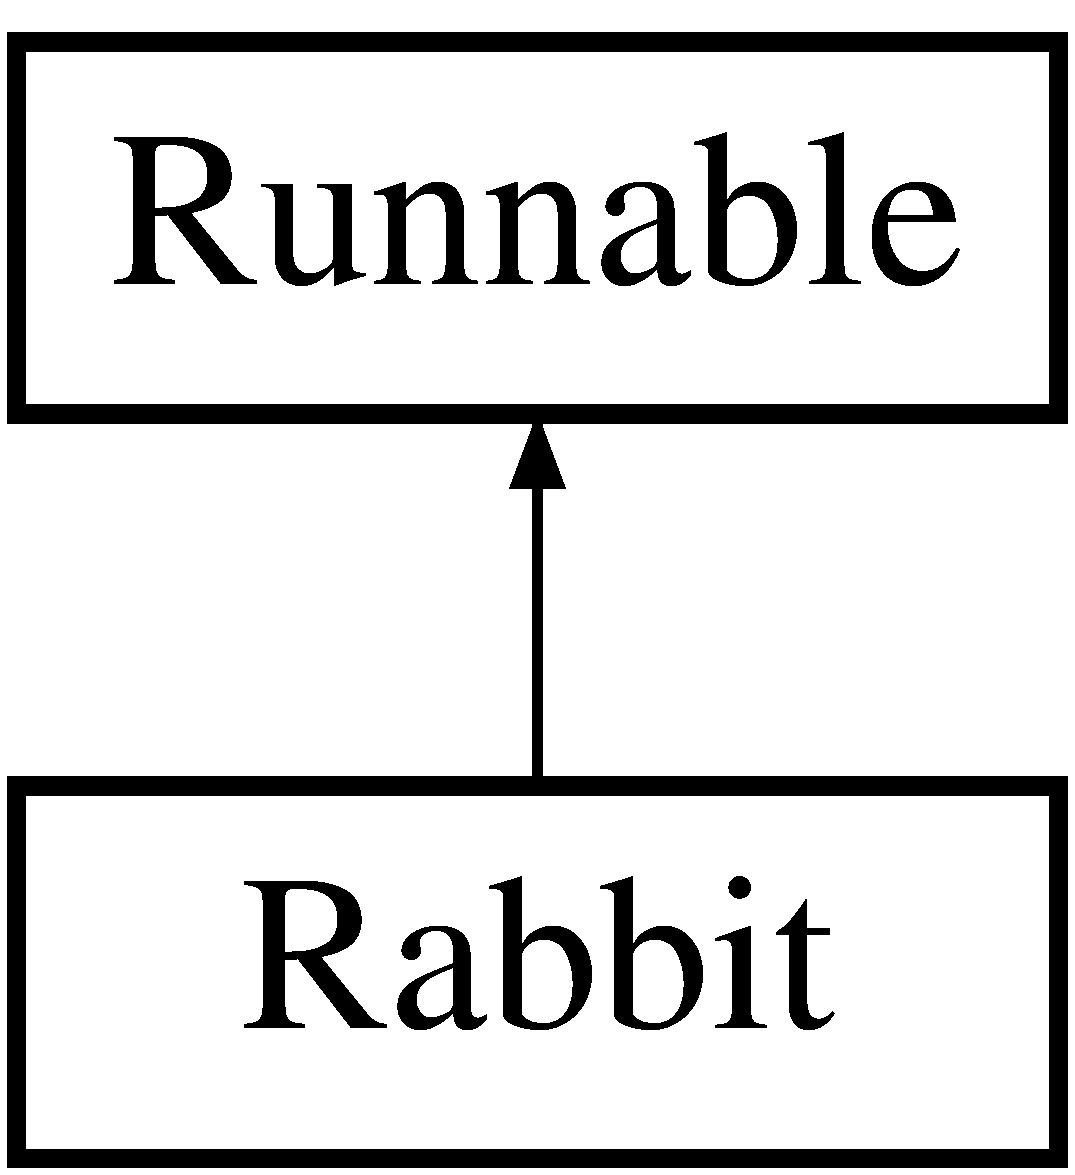
\includegraphics[height=2.000000cm]{class_rabbit}
\end{center}
\end{figure}
\subsection*{Public Member Functions}
\begin{DoxyCompactItemize}
\item 
void \hyperlink{class_rabbit_af83ccda1dd4b52234d28aaffcd0b9bbd}{run} ()
\end{DoxyCompactItemize}


\subsection{Detailed Description}
\hyperlink{class_rabbit}{Rabbit}\textquotesingle{}s class. Is a blueprint for all the rabbits, contains wolf\textquotesingle{}s information to know where to run away. 

\subsection{Member Function Documentation}
\mbox{\Hypertarget{class_rabbit_af83ccda1dd4b52234d28aaffcd0b9bbd}\label{class_rabbit_af83ccda1dd4b52234d28aaffcd0b9bbd}} 
\index{Rabbit@{Rabbit}!run@{run}}
\index{run@{run}!Rabbit@{Rabbit}}
\subsubsection{\texorpdfstring{run()}{run()}}
{\footnotesize\ttfamily void Rabbit.\+run (\begin{DoxyParamCaption}{ }\end{DoxyParamCaption})}



The documentation for this class was generated from the following file\+:\begin{DoxyCompactItemize}
\item 
src/\hyperlink{_rabbit_8java}{Rabbit.\+java}\end{DoxyCompactItemize}

\hypertarget{class_wolf}{}\section{Wolf Class Reference}
\label{class_wolf}\index{Wolf@{Wolf}}
Inheritance diagram for Wolf\+:\begin{figure}[H]
\begin{center}
\leavevmode
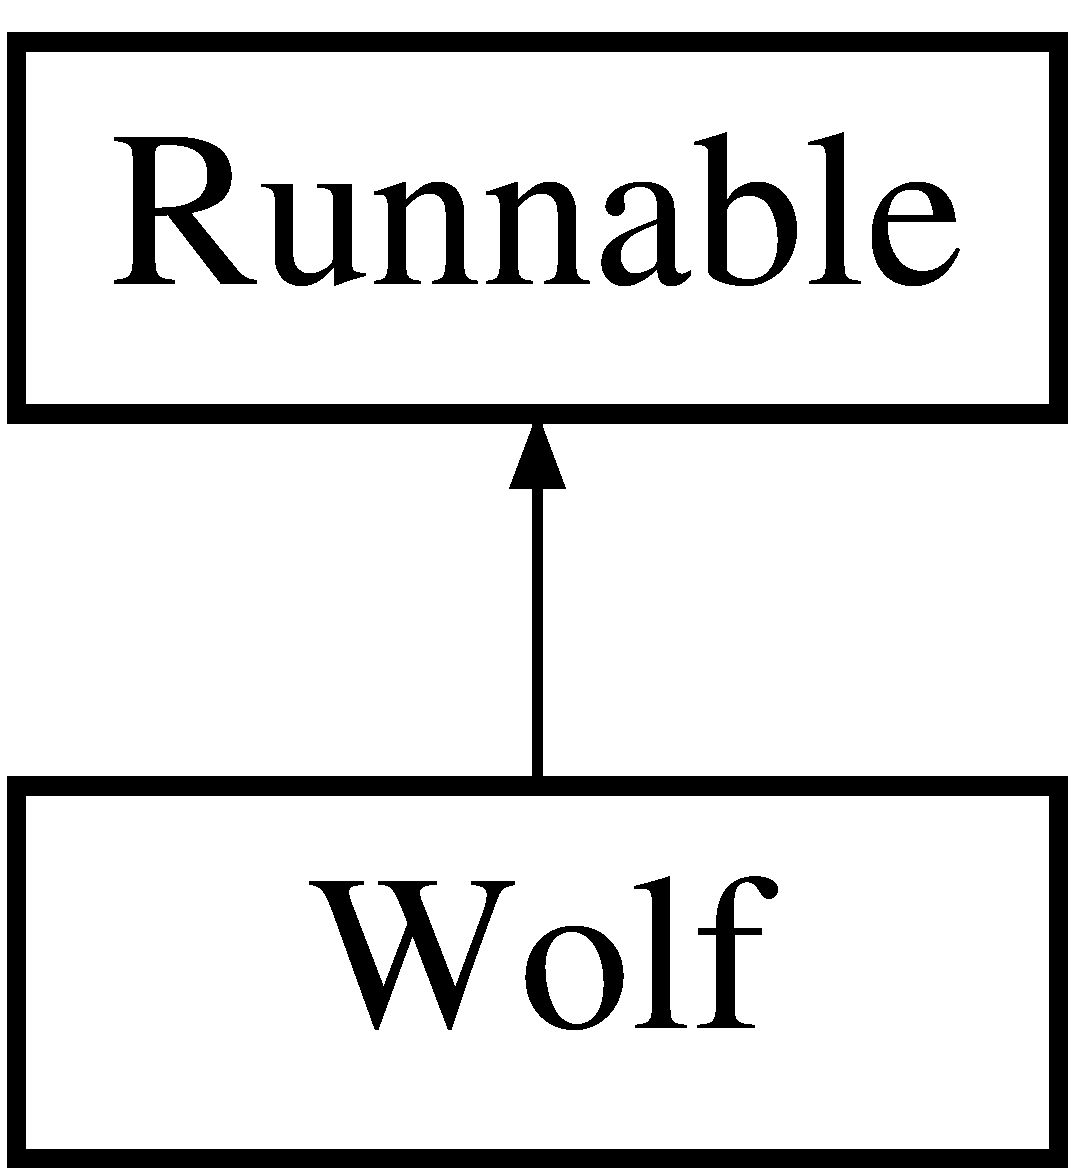
\includegraphics[height=2.000000cm]{class_wolf}
\end{center}
\end{figure}
\subsection*{Public Member Functions}
\begin{DoxyCompactItemize}
\item 
void \hyperlink{class_wolf_ad13213f9167d4afd7abf79eacbf1e74a}{run} ()
\end{DoxyCompactItemize}


\subsection{Detailed Description}
\hyperlink{class_wolf}{Wolf}\textquotesingle{}s class. Contains list of rabbit coordinates to monitor where to move. 

\subsection{Member Function Documentation}
\mbox{\Hypertarget{class_wolf_ad13213f9167d4afd7abf79eacbf1e74a}\label{class_wolf_ad13213f9167d4afd7abf79eacbf1e74a}} 
\index{Wolf@{Wolf}!run@{run}}
\index{run@{run}!Wolf@{Wolf}}
\subsubsection{\texorpdfstring{run()}{run()}}
{\footnotesize\ttfamily void Wolf.\+run (\begin{DoxyParamCaption}{ }\end{DoxyParamCaption})}



The documentation for this class was generated from the following file\+:\begin{DoxyCompactItemize}
\item 
src/\hyperlink{_wolf_8java}{Wolf.\+java}\end{DoxyCompactItemize}

\chapter{File Documentation}
\hypertarget{animation_panel_8java}{}\section{src/animation\+Panel.java File Reference}
\label{animation_panel_8java}\index{src/animation\+Panel.\+java@{src/animation\+Panel.\+java}}
\subsection*{Classes}
\begin{DoxyCompactItemize}
\item 
class {\bfseries animation\+Panel}
\end{DoxyCompactItemize}

\hypertarget{_main_8java}{}\section{src/\+Main.java File Reference}
\label{_main_8java}\index{src/\+Main.\+java@{src/\+Main.\+java}}
\subsection*{Classes}
\begin{DoxyCompactItemize}
\item 
class \hyperlink{class_main}{Main}
\end{DoxyCompactItemize}

\hypertarget{_rabbit_8java}{}\section{src/\+Rabbit.java File Reference}
\label{_rabbit_8java}\index{src/\+Rabbit.\+java@{src/\+Rabbit.\+java}}
\subsection*{Classes}
\begin{DoxyCompactItemize}
\item 
class \hyperlink{class_rabbit}{Rabbit}
\end{DoxyCompactItemize}

\hypertarget{_wolf_8java}{}\section{src/\+Wolf.java File Reference}
\label{_wolf_8java}\index{src/\+Wolf.\+java@{src/\+Wolf.\+java}}
\subsection*{Classes}
\begin{DoxyCompactItemize}
\item 
class \hyperlink{class_wolf}{Wolf}
\end{DoxyCompactItemize}

%--- End generated contents ---

% Index
\backmatter
\newpage
\phantomsection
\clearemptydoublepage
\addcontentsline{toc}{chapter}{Index}
\printindex

\end{document}
